%\documentclass[a4paper, 11pt, addpoints]{exam}
%%\documentclass[a4paper, 11pt, addpoints, answers]{exam}  % Desconmente esta linha, para ver as respostas, e comente a de cima
%\usepackage{listaufersa}
%\usepackage{listings} % Mostrar código-fonte
%\usepackage[brazil]{babel}
%\usepackage{multicol}
%\usepackage{booktabs}
%\usepackage{hyperref}
%
%\setlength{\columnsep}{25pt}
%\lstdefinestyle{js}{
%    basicstyle=\ttfamily,
%    breaklines=true,
%    breakatwhitespace=true,
%    tabsize=1,
%    resetmargins=true,
%    xleftmargin=0pt,
%    frame=none
%}
%
%
%
%
%%%%%%%%%%%%%%%%%%%%%%%%%%%%%%%%%%%%%%%%%%%%%%%%%%
%
%\pointpoints{Ponto}{Pontos}
%
%\begin{document}


%%%%%%%%% Informações sobre o curso %%%%%%%%%%%%%

%
%\nomeProfessor{Rodrigo Toledo Teixeira Câmara}
%\nomeCurso{Bacharelado em Ciências e Tecnologias}
%\nomeDisciplina{Cálculo Numérico}
%\semestre{5}   % Deixe em branco se for para mais de um semestre (recuperação)
%\dataDaProva{2016.2}
%\tipoAvaliacao{lista da aula 05}
%
%\info
%\vspace{-0.5 cm}
%

%%%%%%%%%%%%%%%%%%%%%%%%%%%%%%%%%%%%%%%%%%%%%%%%%



%\begin{questions}
%\begin{multicols}{2}


\begin{ex}\label{jacobi}
Faça os testes do critério das linhas nos seguintes sistemas lineares. Se a convergência for satisfeita, faça as duas primeiras iterações do método de Gauss-Jacobi. Ao final de cada iteração, calcule $d^{(k)}$, $d_r^{(k)}$ e $|Ax^{(k)}-b|$.
\begin{enumerate}
\item $\begin{cases}
2x+3y+z=11\\
x+y+z=6\\
5x+2y+3z=18
\end{cases}.$
\item $\begin{cases}
5x+y+z=7\\
2x+6y-2z=6\\
y+2z=3
\end{cases}.$
\item $\begin{cases}
4x-y+7z=9\\
5x+3y-z=0\\
-7x-11y+17z=19
\end{cases}.$
\item $\begin{cases}
x+6y+z=8\\
2x-6z=-4\\
3x+y=4
\end{cases}.$
\end{enumerate}
\begin{sol}
\begin{enumerate}
\item A análise pelo critério das linhas é inconclusiva.
\item De acordo com o critério das linhas, o método de Gauss-Jacobi gera uma sequência convergente. 


Partindo da solução inicial $x^{(0)}=\begin{bmatrix}
0&0&0
\end{bmatrix}^t$, as candidatas a solução são $x^{(1)}=\begin{bmatrix}
1.4&1&1.5
\end{bmatrix}^t$ e $x^{(2)}=\begin{bmatrix}
0.9&1.033&1
\end{bmatrix}^t$.

$d^{(1)}=1.5, d^{(2)}=0.5, d_r^{(1)}=1,d_r^{(2)}=0.484$.

$||Ax^{(1)}-b||_\infty=2.5, ||Ax^{(2)}-b||_\infty=0.467$.
\end{enumerate}

%\begin{enumerate}
%\item $\begin{bmatrix}
%12&9\\18&45
%\end{bmatrix}$
%\item $\begin{bmatrix}
%14&7\\32&43
%\end{bmatrix}$
%\item $\begin{bmatrix}
%14\\5\\4
%\end{bmatrix}$
%\item Não é possível calcular.
%\end{enumerate}
\end{sol}
\end{ex}

\begin{ex}
Refaça a questão \ref{jacobi}, mas desta vez testando a convergência com o critério de Sassenfeld. Caso a convergência seja satisfeita, calcule as duas primeiras iterações do método de Gauss-Seidel.
\begin{sol}
\begin{enumerate}
\item A análise pelo critério de Sasenfeld é inconclusiva.
\item De acordo com o critério de Sassenfeld, o método de Gauss-Seidel gera uma sequência convergente.

Partindo da aproximação inicial $x^{(0)}=\begin{bmatrix}
0&0&0
\end{bmatrix}^t$, temos $x^{(1)}=\begin{bmatrix}
1.4& 0.5333 &1.2333
\end{bmatrix}^t$ e $x^{(2)}=\begin{bmatrix}
1.0467& 1.0622 &0.9689
\end{bmatrix}^t$.
\end{enumerate}
\end{sol}
\end{ex}


\begin{ex}
Com o auxílio do \emph{Visual Cálculo Numérico}, calcule as soluções dos sistemas da questão \ref{jacobi} por meio do método de Gauss-Jacobi e por meio do método de Gauss-Seidel, \emph{caso a respectiva convergência seja garantida}. Em todos os casos, utilize a precisão $\epsilon=0.1$ com o critério de parada de sua preferência.
\end{ex}

\section{Problemas}
%\end{questions}


\begin{ex}
Uma função \emph{polinomial de segundo grau} é uma função no formato
\begin{equation}\label{poli}
p_2(x)=ax^2+bx+c,
\end{equation}
com $a\neq 0$. 


Encontre a função polinomial de segundo grau cujo gráfico passa pelos pontos $(1;5)$, $(3;11)$ e $(5;25)$. Em seguida, trace o gráfico desta função no \emph{GeoGebra} e confirme se de fato este passa pelos pontos dados.


Dica: Observe que, pela equação \ref{poli}, um ponto, digamos $(x_0;y_0)$, pode ser representado pela equação linear
$$p_2(x_0)=ax_0^2+bx_0+c,$$
onde $p_2(x_0)=y_0$.
\end{ex}
\begin{ex}
Considere o circuito elétrico%\footnote{Retirado de \emph{Cálculo Numérico}, de BURIAN, LIMA e HETEM JÚNIOR, coleção Fundamentos de Informática.} 
 representado na figura \ref{circuitoburian}.
\begin{figure}[htb]
\caption{Circuito elétrico formado por três resistores e uma bateria de 12 volts.}
\label{circuitoburian}
\begin{center}
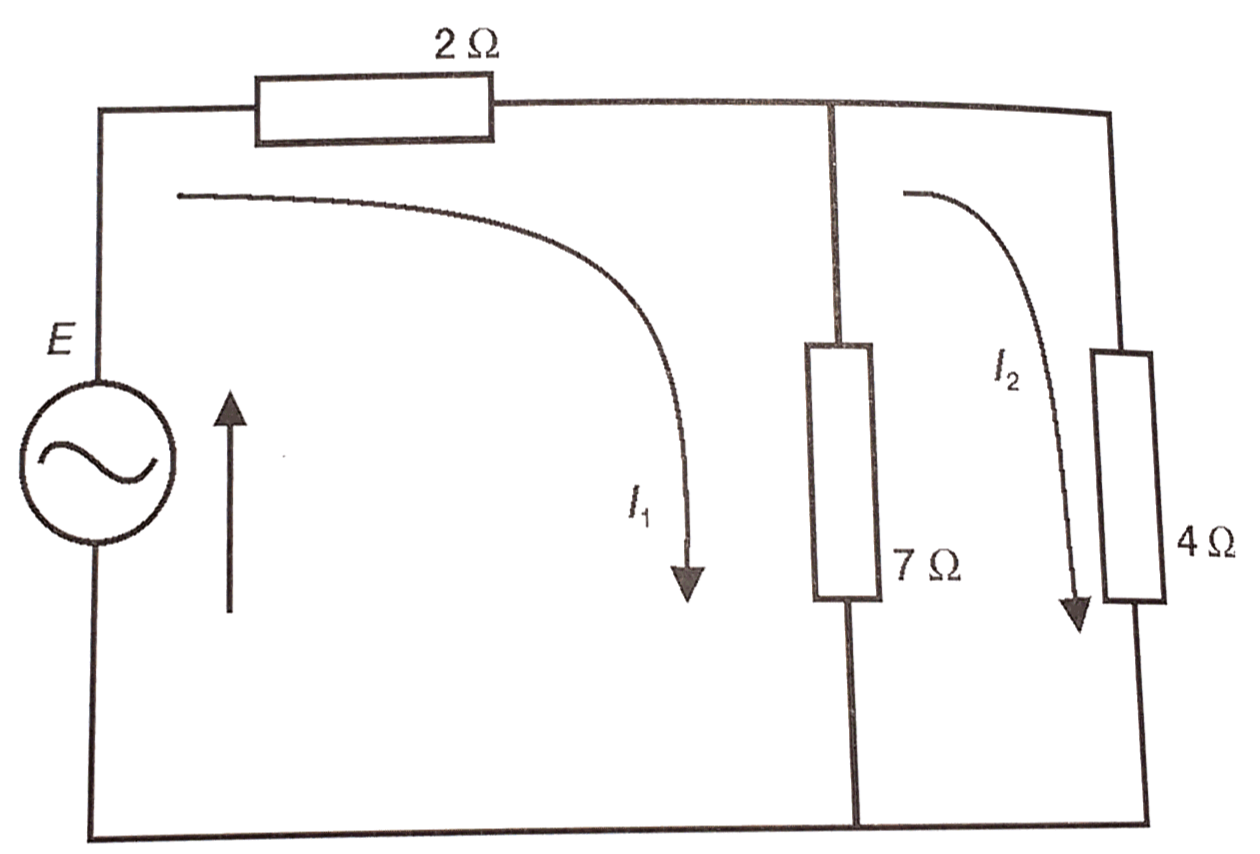
\includegraphics[width=0.5\linewidth]{fig/circuitoburian}
\end{center}
\end{figure}
Pela Lei das Malhas, este circuito pode ser modelado pelo sistema linear
$$\begin{cases}
2i_1+7i_1-7i_2=12\\
7i_2+4i_2-7i_1=0
\end{cases}.$$
Determine, em amperes, as intensidades das correntes neste circuito.
\end{ex}

\begin{ex}\label{ex.forno}
Um grande forno industrial é suportado por uma longa coluna de tijolos refratários. Durante a operação, as condições são tais que três superfícies da coluna são mantidas a temperaturas altas. 

É de interesse dos responsáveis da indústria que a temperatura dos tijolos seja calculada, a fim de auxiliar na escolha dos materiais e traçar estratégias sobre a segurança dos funcionários da indústria, sobre a manutenção do equipamento e sobre a eficiência energética.


O problema do cálculo das temperaturas pode ser simplificado da seguinte forma: primeiro, divida a área da coluna em retângulos, conforme a figura \ref{fig.forno}. Em seguida, analise a temperatura somente nos \emph{pontos nodais}, ou seja, nos vértices dos retângulos.

\begin{figure}[hb]
\center
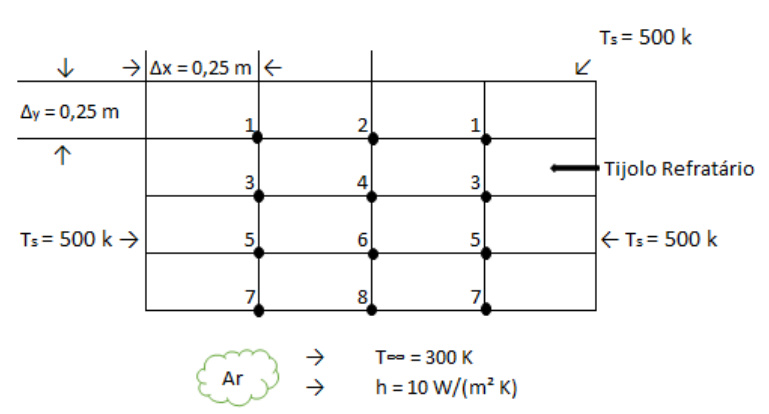
\includegraphics[width=0.8\linewidth]{forno}
\caption{Esquema que indica os 12 pontos nodais que devem-se calcular a temperatura.}\label{fig.forno}
\end{figure}

Pela simetria do forno, basta calcular a temperatura apenas dos pontos nodais 1, 2, 3, 4, 5, 6, 7 e 8. As temperaturas destes pontos são, respectivamente, $T_1, T_2, T_3, T_4, T_5, T_6, T_7$ e $T_8$.


De acordo com a termodinâmica, as temperaturas $T_1, T_3$ e $T_5$ dos pontos ``interiores'' 1, 3 e 5 podem ser descritas pelas equações
\begin{align*}
4T_1&=T_2+T_3+1000\\
4T_3&=T_1+T_4+T_5+500\\
4T_5&=T_3+t_6+T_7+500.
\end{align*}

Já para os nós 2, 4 e 6, que são do tipo ``ponto nodal em uma superfície adiabática plana com convecção'', as temperaturas são descritas, respectivamente, pelas equações
\begin{align*}
4T_2&=2T_1+T_4+500\\
4T_4&=T_2+2T_3+T_6\\
4T_6&=T_4+2T_5+T_8.
\end{align*}


Por último, as temperaturas dos nós 7 e 8, do tipo ``ponto nodal em uma superfície não-adiabática, plana, com convecção'' localizados na parte inferior da coluna, podem ser
descritas pelas equações
\begin{align*}
9T_7&=2T_5 + T_8 + 2000\\
9T_8&=2T_6 + 2T_7 + 1500.
\end{align*}

Determine as temperaturas $T_1, T_2, T_3, T_4, T_5, T_6, T_7$ e $T_8$ dos nós.
\end{ex}

\begin{ex}
Considere a reação estequiométrica entre $x$ mols de ácido clorídrico ($HCl$) e $y$ mols de ácido
perclórico ($HClO_3$), que tem como produtos $z$ mols de dióxido de monocloro ($ClO_2$) e $w$
mols de água ($H_2O$):
$$xHCl+yKClO_3\rightarrow zClO_2+wH_2O.$$


Supondo que essa reação produziu $3$ mols de água, modele um sistema linear que descreve
as quantidades de mols das demais substâncias e as determine. Dica: as quantidades de $H$, de $Cl$ e
de $O$ antes da seta devem ser iguais às quantidades de depois da seta (``Nada se cria, nada
se perde, tudo se transforma'', Lavoisier).
\label{ex.quimica}\end{ex}

%\end{document}

% \begin{ex}
% Considere o circuito da figura \ref{circ}
% \begin{figure}[!htb]
% \begin{center}
% \label{circ}
% 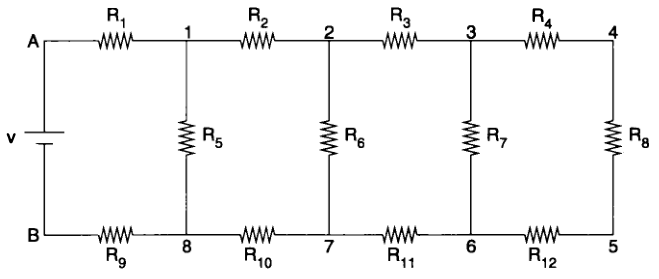
\includegraphics[width=0.6\linewidth]{fig/circuitoexercicio.png}
% \caption{Circuito elétrico de oito nós.}
% \end{center}
% \end{figure}
% Considerações:
% \begin{enumerate}
% \item Os parâmetros do circuito são:\\$R_1=1, R_2=2, R_3=1, R_4=3, R_5=5, R_6=2, R_7=6, R_8=1, R_9=2, R_{10}=3, R_{11}=8, R_{12}=8,$\\
% $V_A=100, V_B=0$.
% % \item A corrente elétrica de um nó $p$ para um nó $q$ é dada por
% % $$I_{pq}=\frac{V_p-V_q}{R_{pq}}$$
% % onde $V_p$ e $V_q$ são as tensões (volts) nos nós $p$ e $q$ respectivamente e $R_{pq}$ é a resistência (em ohms) entre os nós $p$ e $q$.
% \item Pela lei de Kirchoff, a soma algébrica das correntes em cada ciclo é zero.
% \end{enumerate}
% Modelagem do problema:\\
% Em cada ramo associamos um sentido qualquer. Para os ramos A18B, 1276, 2367 e 3456 atribuímos o sentido horário, por exemplo. Pela lei dos nós, temos para o ramo A18B que
% $$R_1*I_{A,1}+R_5*I_{1,8}+R_9*I_{8,B}=V_{A,B}.$$
% Atribuindo os respectivos valores, temos que
% $$1I_{A,1}+5I_{1,8}+2I_{8,B}=100,$$
% que é uma equação linear.

% Para o ramo 1278 atribuímos o sentido horário. Desta forma, o cálculo da corrente pode ser modelada como
% $$R_2*I_{12}+R_6*I_{27}$$


% \begin{enumerate}
% \item Modele o sistema linear que relaciona as correntes neste circuito.
% \item Resolva o sistema linear com o \emph{Visual Cálculo Numérico} com o método que você achar mais apropriado.
% \end{enumerate}


% \end{ex}

%\end{questions}

%\end{document}